\documentclass[tikz,border=5pt]{standalone}
\usepackage{fontspec}
\setmainfont{Times New Roman}
\usepackage{unicode-math}
\setmathfont{Cambria Math}
\usetikzlibrary{shapes.geometric,positioning,fit,backgrounds,arrows.meta,calc}

\begin{document}
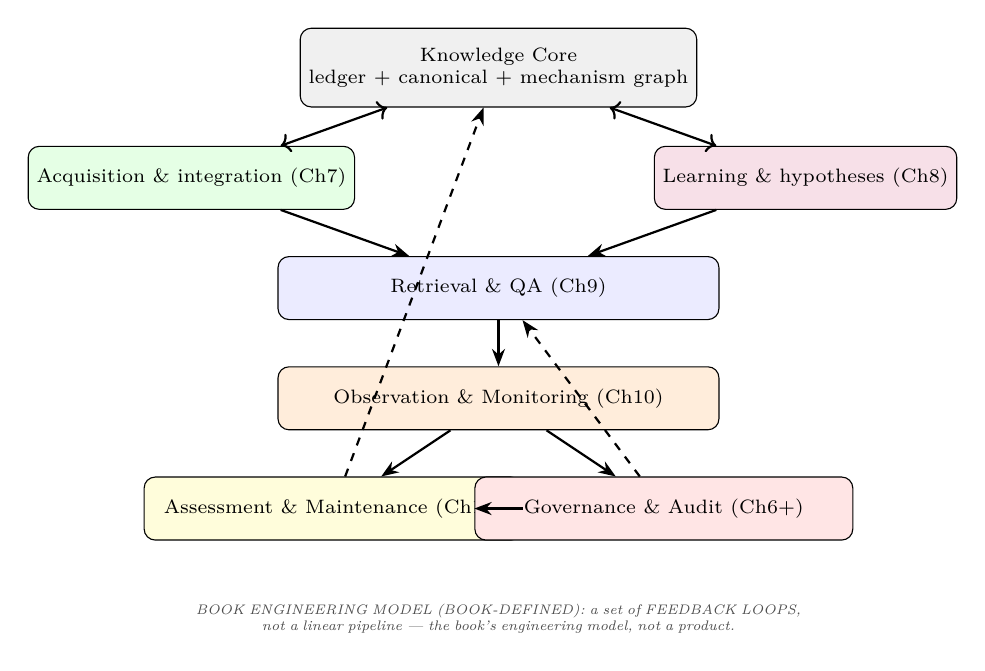
\begin{tikzpicture}[
  box/.style={rectangle, draw, rounded corners, align=center, font=\scriptsize, inner sep=3pt},
  arrow/.style={-{Stealth[length=2.2mm]}, thick},
  label/.style={font=\tiny\itshape, text=gray!60!black},
]

% === LIVING ARCHITECTURE (BOOK ENGINEERING MODEL) ===
\node[box, fill=gray!12, minimum width=3.6cm, minimum height=1.0cm] (core) at (0, 4.6) {Knowledge Core\\ledger + canonical + mechanism graph};

\node[box, fill=green!10, minimum width=3.6cm, minimum height=0.8cm] (acq) at (-3.9, 3.2) {Acquisition \& integration (Ch7)};
\node[box, fill=purple!12, minimum width=3.6cm, minimum height=0.8cm] (lrn) at (3.9, 3.2) {Learning \& hypotheses (Ch8)};

\node[box, fill=blue!8, minimum width=5.6cm, minimum height=0.8cm] (qa) at (0, 1.8) {Retrieval \& QA (Ch9)};

\node[box, fill=orange!14, minimum width=5.6cm, minimum height=0.8cm] (obs) at (0, 0.4) {Observation \& Monitoring (Ch10)};

\node[box, fill=yellow!14, minimum width=4.8cm, minimum height=0.8cm] (mnt) at (-2.1, -1.0) {Assessment \& Maintenance (Ch10)};
\node[box, fill=red!10, minimum width=4.8cm, minimum height=0.8cm] (gova) at (2.1, -1.0) {Governance \& Audit (Ch6+)};

\draw[<->, thick] (core) -- (acq);
\draw[<->, thick] (core) -- (lrn);
\draw[arrow] (acq) -- (qa);
\draw[arrow] (lrn) -- (qa);
\draw[arrow] (qa) -- (obs);
\draw[arrow] (obs) -- (mnt);
\draw[arrow] (obs) -- (gova);
\draw[arrow] (mnt) -- (gova);
\draw[arrow, dashed] (mnt) -- (core);
\draw[arrow, dashed] (gova) -- (qa);

\node[label, align=center, text width=11cm] at (0, -2.4)
  {BOOK ENGINEERING MODEL (BOOK-DEFINED): a set of FEEDBACK LOOPS,\\not a linear pipeline — the book's engineering model, not a product.};
\end{tikzpicture}
\end{document}
